\subsection{Giao tiếp nội bộ -- TCP NestJS, mTLS và xác thực dữ liệu đầu vào}

Các dịch vụ nội bộ của hệ thống giao tiếp với nhau qua \textbf{NestJS TCP transport} thay vì REST HTTP. Cách làm này loại bỏ tầng parser HTTP, giảm độ trễ trung bình từ 5--15 ms xuống còn 1--3 ms cho mỗi vòng gọi, và quan trọng hơn -- các dịch vụ ngoài BFF và Reveal-Vote không cần mở cổng HTTP, do đó không trực tiếp tiếp xúc với mạng bên ngoài. Sơ đồ giao tiếp tổng thể được minh họa trong Hình~\ref{fig:internal-services}.

\textbf{mTLS cho kênh TCP giữa các microservice:} Do các microservice có thể được triển khai trên các máy chủ khác nhau và giao tiếp thông qua hạ tầng mạng không hoàn toàn tin cậy, hệ thống sử dụng \textit{mutual TLS} (mTLS) để mã hóa dữ liệu truyền tải và xác thực hai chiều danh tính dịch vụ. Nhờ đó, chỉ những dịch vụ sở hữu chứng chỉ hợp lệ mới có thể tham gia trao đổi dữ liệu. Cấu hình microservice của NestJS được khởi tạo với \pkg{tlsOptions}:

\begin{figure}[H]
    \centering
    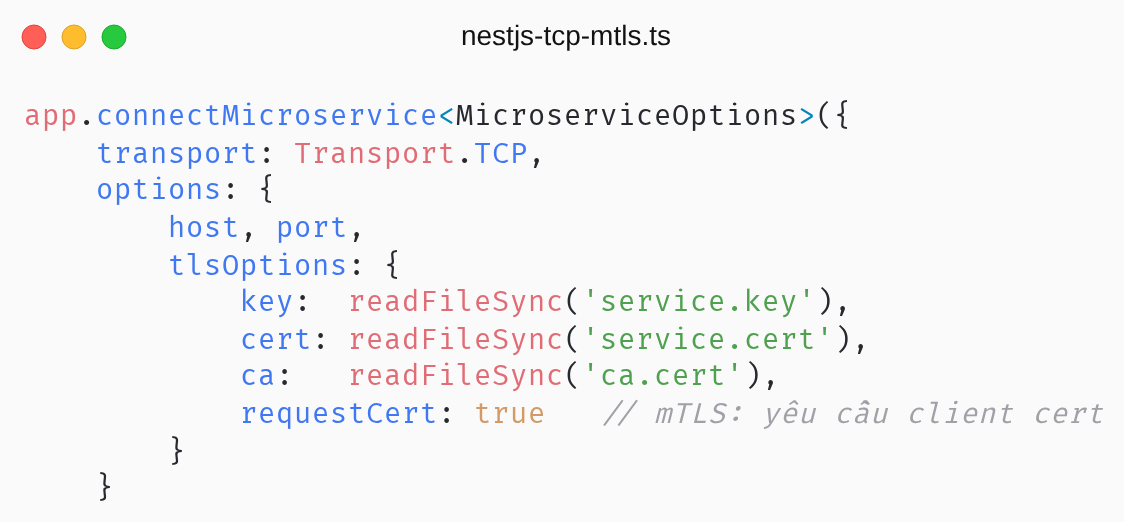
\includegraphics[width=0.75\textwidth, keepaspectratio]{Figures/code/nestjs-tcp-mtls.png}
    \caption{Cấu hình mTLS cho NestJS TCP microservice với tlsOptions}
    \label{fig:nestjs-tcp-mtls}
\end{figure}

\textbf{Xác thực dữ liệu đầu vào:} Mọi yêu cầu vào hệ thống -- cả từ trình duyệt qua HTTP đến BFF lẫn từ microservice qua kênh TCP -- đều được kiểm chứng tự động qua \pkg{ValidationPipe} toàn cục. Lớp DTO khai báo các ràng buộc dưới dạng decorator của \pkg{class-validator}: \pkg{@IsDefined}, \pkg{@IsString},... Ví dụ điển hình là \pkg{SignInDto} và \pkg{RefreshTokenDto} trong Hình~\ref{fig:class-validator-dto}.

\begin{figure}[H]
    \centering
    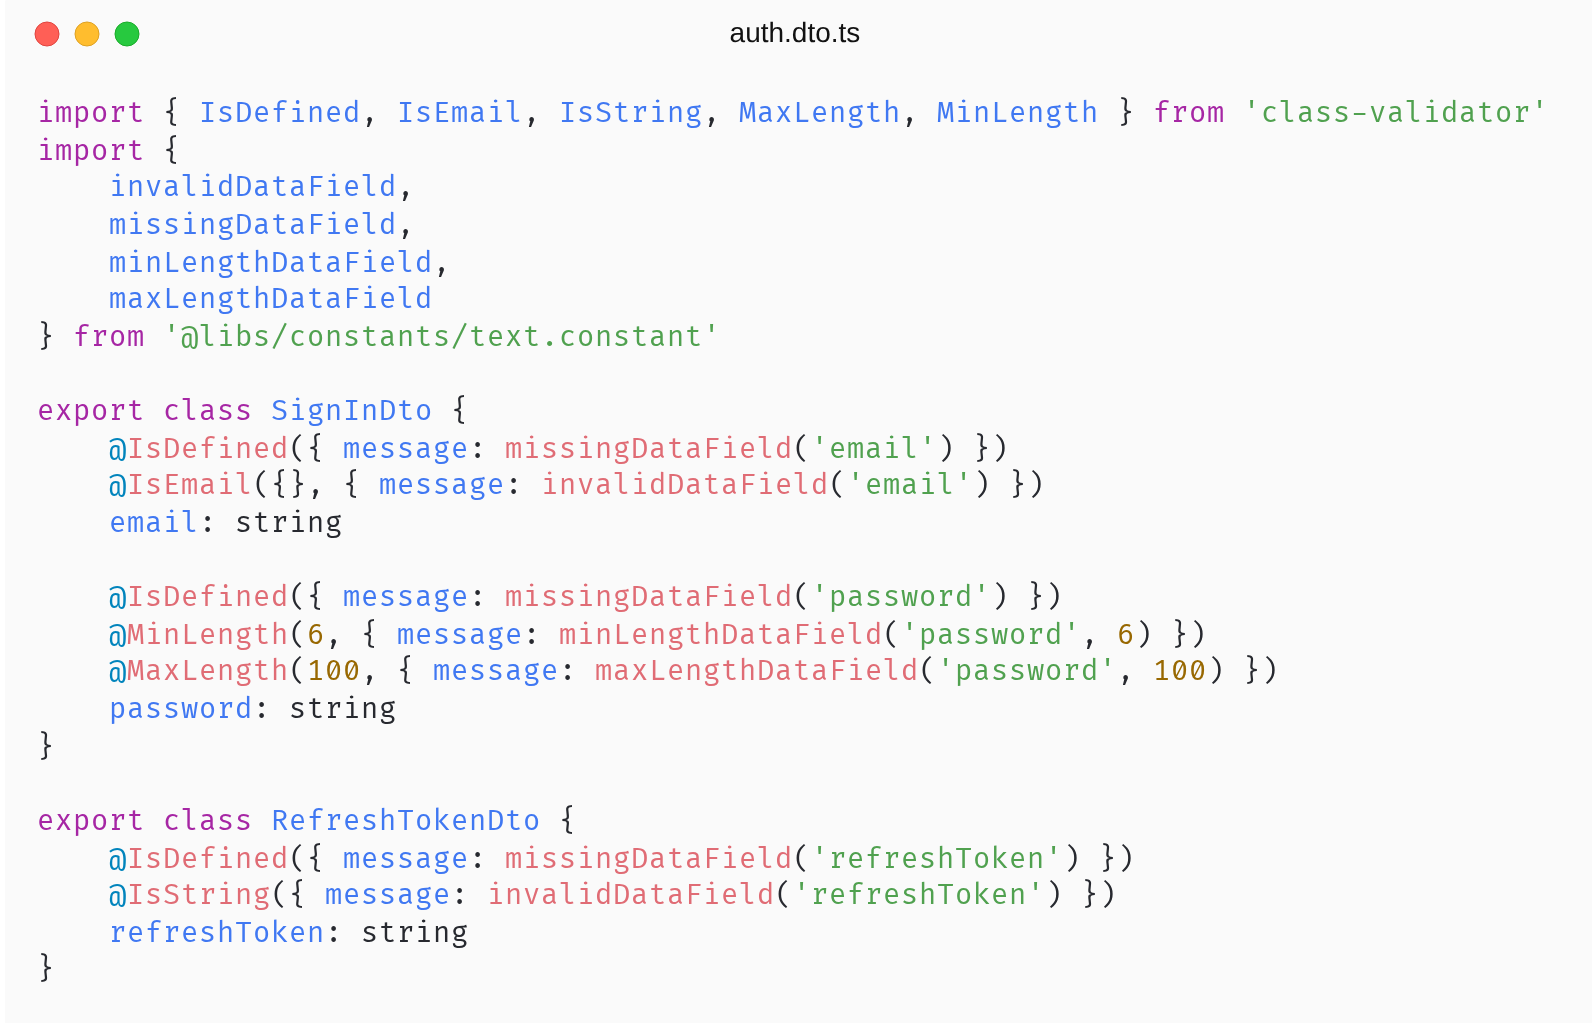
\includegraphics[width=0.85\textwidth, keepaspectratio]{Figures/code/class-validator-dto.png}
    \caption{DTO xác thực dữ liệu vào bằng decorator của class-validator}
    \label{fig:class-validator-dto}
\end{figure}
